\documentclass[a4paper,12pt]{report}
\usepackage[utf8]{inputenc}
\usepackage[swedish]{babel}
\usepackage{hyperref}
\usepackage{graphicx}
\usepackage{csquotes}

\usepackage{gensymb}

\usepackage{pgfplots}
\usepackage{pgfplotstable}
\pgfplotsset{compat=1.14}

\usetikzlibrary{external}
\tikzexternalize[prefix=tikz/]

\usepackage[export]{adjustbox}
\usepackage{wrapfig}
\usepackage{subfig}

\usepackage[parfill]{parskip}

\usepackage{amsmath}

%\usepackage{fancyhdr}
%\fancypagestyle{titlepagestyle}
%{
%   \fancyhf{}
%   \fancyfoot[L]{}%\emph{This text needs to appear on the title %page}}
%   \renewcommand{\headrulewidth}{0 mm}
%}

\usepackage{titling}

\usepackage{titlesec}
\titleformat{\chapter}
  {\normalfont\Large\bfseries}{\thechapter}{1em}{}
% \titleformat{\section}
%  {\normalfont\bfseries}{}{1em}{}
%\titlespacing*{\chapter}{0pt}{3.5ex plus 1ex minus .2ex}{2.3ex plus .2ex}

\makeatletter
\renewcommand\footnotesize{%
   \@setfontsize\footnotesize\@ixpt{11}%
   \abovedisplayskip 8\p@ \@plus2\p@ \@minus4\p@
   \abovedisplayshortskip \z@ \@plus\p@
   \belowdisplayshortskip 4\p@ \@plus2\p@ \@minus2\p@
   \def\@listi{\leftmargin\leftmargini
               \topsep 4\p@ \@plus2\p@ \@minus2\p@
               \parsep 2\p@ \@plus\p@ \@minus\p@
               \itemsep \parsep}%
   \belowdisplayskip \abovedisplayskip
}
\makeatother

%\usepackage{ftnxtra} %\autocite i \caption
\usepackage[backend=bibtex,style=verbose]{biblatex}  % style kan också vara authoryear (el. dyl.)
\DeclareNameAlias{sortname}{family-given}
\renewbibmacro{in:}{}

\addbibresource{referenser.bib}

\begin{document}

\pagenumbering{gobble}

\begin{titlepage}
	\centering
	%\includegraphics[width=0.15\textwidth]{example-image-1x1}\par\vspace{1cm}
	%{\LARGE Blackebergs gymnasium \par}
	%\vspace{1.25cm}
	{\huge\bfseries Undersökning av Vintergatans struktur \par}
	%\vspace{0.5cm}
	%{\large Appbygge med användning av metodik för att främja användarvänlighet \par}
	\vfill
	{\Large\begin{tabular}{c c}
	     Gustav Sörnäs & Vilhelm Larsson  \\
	     Blackebergs gymnasium & Bromma gymnasium \\
	     Na16c & T16
	\end{tabular}\par}
	\vfill
	Handledare:\par
	Christina \textsc{Kronlund} - Bromma gymnasium\\
	Karin \textsc{Enström Salomonsson} - Bromma gymnasium\\
	Simon \textsc{Eriksson} - Institutionen för Astronomi - Stockholms Universitet\\
	Thomas \textsc{Pettersson} - Blackebergs gymnasium

	\vfill

% Bottom of the page
	{\large \today\par}
\end{titlepage}

\newpage
\pagenumbering{roman}

\chapter*{Abstract}
This report aims to answer one main question and one minor question regarding the galactic aspect of the Milky Way. How is the Milky Way structured, and why are galaxies structured in the way that they are? To answer the first question we use a radio telescope which detects hydrogen. Hydrogen is the most common form of matter in the known universe, and by using the aforementioned telescope and calculating the Doppler effect backwards, we can estimate how much hydrogen there is at every given point in the sky. We use galactic coordinates to determine the position of ''clouds'' of hydrogen, and after we process the data through several steps we can also place the ''clouds'' on the galactic scale, and therefore map our galaxy. We also explore the current explanations as to why galaxies assume certain structures by presenting current scientific theories regarding the matter.

\newpage

\tableofcontents

\listoffigures

\newpage
\pagenumbering{arabic}

\chapter{Inledning}

Det synliga universums massa består av mellan 70\% och 80\% väte. På grund av gravitation ansamlas vätet i vätemoln av olika storlekar. Vårt arbete utnyttjar en välkänd mekanism hos väte, en så kallad ''Spin-Flip Transition''\autocite{swin.edu:spin-flip}. Väteatomer består av en proton och en elektron. Dessa partiklar har en kvantmekanisk spin (som kallas spin även om partiklarna inte snurrar enligt den klassiska fysikens definition av spin). I basläget (det läge med lägst energinivå) har elektronen och protonen motsatt spin mot varandra. Om elektronen i väteatomen tar emot energi (vilket kan ske spontant genom exempelvis kollisioner mellan atomer) kan elektronen byta spin och få samma spin som protonen. Detta läge har marginellt högre energinivå än basläget. Om elektronen sedan byter till motsatt spin igen kommer överskottsenergin avges i form av en foton med en våglängd på ungefär 21cm. Denna våglängd kan vi observera med hjälp av ett radioteleskop här på jorden.

\section{Dopplereffekten}
Alla vågrörelser påverkas av dopplereffekten\autocite{nasa:doppler}. Dopplereffekten uppstår när en sändare som skickar ut någon form av vågrörelse har en hastighet riktad antingen mot eller från mottagaren. Om sändaren rör sig bort från mottagaren kommer våglängden bli längre (vågen ''sträcks ut'') och om sändaren rör sig mot mottagaren blir vågländen kortare (vågen ''trycks ihop''). 

I vår vardag upplevs dopplereffekten mest med ljudvågor. Om en observatör lyssnar på ett utryckningsfordon som åker förbi med sirenerna på kommer observatören notera att ljudet låter ljusare när sirenerna närmar sig och när sirenerna passerat observatören kommer ljudet låta mörkare. Givet formeln för dopplereffekten \autocite{wikipedia:doppler} 
\begin{equation*}
    \frac{f}{v_{wr}} = \frac{f_0}{v_{ws}}
\end{equation*}
kan vi räkna ut den upplevda  förskjutningen $x$ i frekvens genom 
\begin{align*}
    f &= f_0 \cdot x \\
    f &= \frac{f_0 \cdot v_{wr}}{v_{ws}} \Rightarrow x = \frac{v_{wr}}{v_{ws}}.
\end{align*}

Om vi tänker oss en ambulans med en hastighet 30m/s och en uppskattad ljudhastighet i luft på 300m/s kommer sirenens frekvens dopplerförskjutas till $f_0 \cdot \frac{300}{300-30}$, alltså 10\% högre än den sändes ut med. Ljuset som skickas ut från ambulansens varningsljus kommer också förskjutas men på grund av ljusets höga hastighet (runt 300 000 000 m/s) kommer ljusets frekvens endast öka med ungefär 0,00001\%.

\begin{figure}
    \centering
    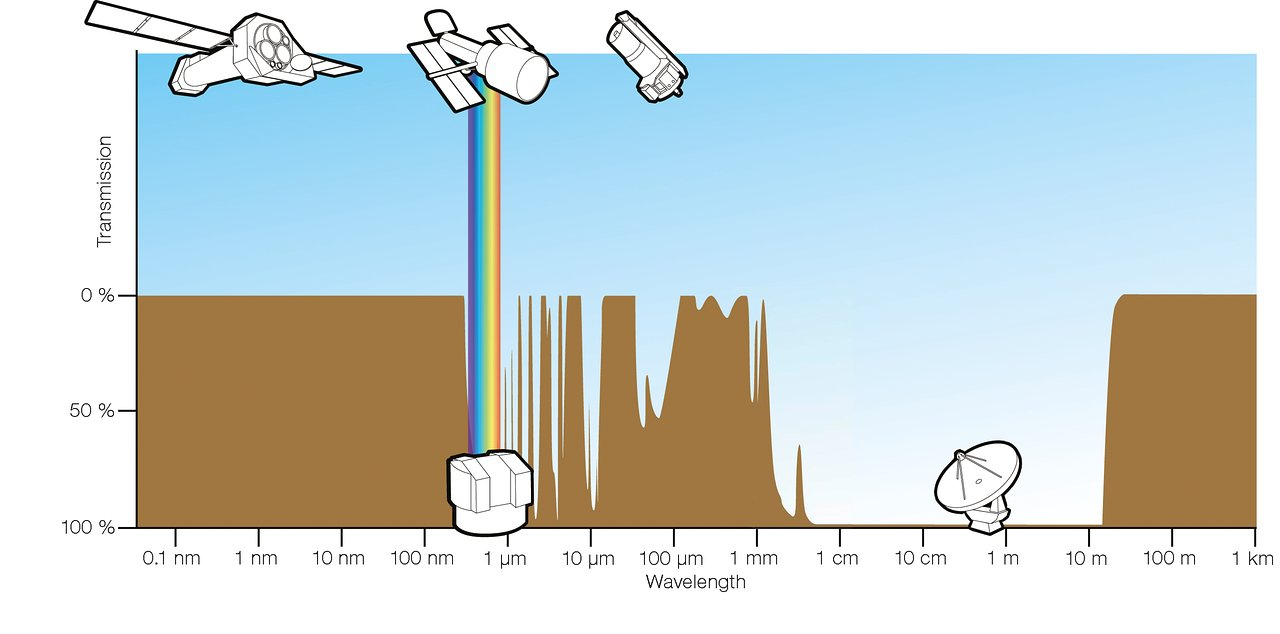
\includegraphics{pics/atmo.jpg}
    \caption{Atmosfärens genomskinlighet för olika våglängder av ljus.}
    \label{fig:atmo_transparent}
\end{figure}

\section{Att observera rymden}
Förutom radiovågor görs astronomiska observationer på gamma- och röntgen-strålning, ultraviolett strålning, synligt ljus, infraröd strålning samt mikrovågor. Av dessa olika typer av ljus släpps enbart synligt ljus och radiovågor genom atmosfären (se figur \ref{fig:atmo_transparent}). Radiovågor passerar relativt ostört genom hela atmosfären \autocite{nasa:radiowaves}, så även om synligt ljus passerar störs det lätt av exempelvis moln \autocite{wikipedia:astro_seeing}. För övriga signaltyper används istället diverse satelliter i omloppsbana kring jorden.

\begin{figure}
    \centering
    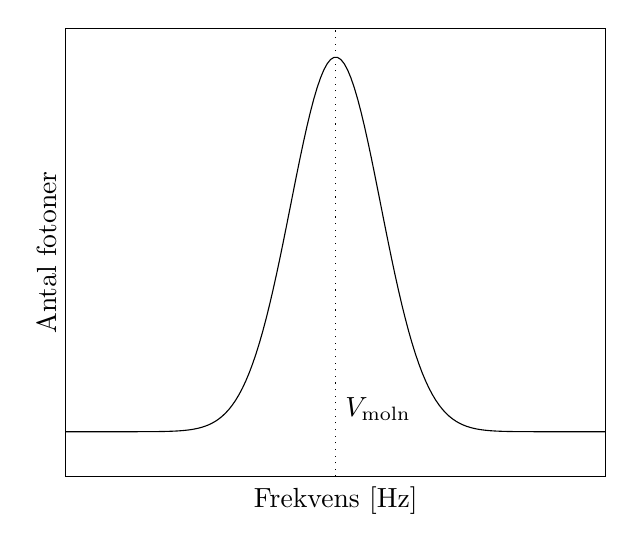
\begin{tikzpicture}
        \begin{axis}[
            ticks=none,
            ylabel=Antal fotoner, ylabel near ticks,
            xlabel={Frekvens [Hz]}, xlabel near ticks,
            xmin=-20, xmax=20,
            ymin=-1, ymax=9
        ]
        \addplot [domain=-25:25, samples=200]{1/0.3*(2*pi)^0.5 * exp(-((x)^2)/2*0.09)};
        \addplot [black, dotted] coordinates {
            (0,-1)
            (0,9)
        };
        \coordinate [label=right:$V_{\mathrm{moln}}$] (v-label) at (0,0.5);
        \end{axis}
    \end{tikzpicture}
    \caption{En exempelmätning med ett observerat vätemoln.}
    \label{fig:single_cloud}
\end{figure}

När vi gör en observation mäter vi i praktiken antalet fotoner inom ett visst spann av våglängder. Om vi tänker oss väte ansamlat i ''moln'' av olika storlekar i Vintergatan kommer molnet ha en viss hastighet med en riktning som följer Vintergatans rotation. Däremot kommer de enskilda atomerna som skickar ut fotonerna vi mäter ha olika relativa hastigheter där några kommer åka lite mer mot oss och några lite mer bort från oss. På grund av detta kommer antalet fotoner med olika våglängder spridas ut över ett visst intervall, men en majoritet av fotonerna kommer vara relativt stilla gentemot molnet (se figur \ref{fig:single_cloud}).

\begin{figure}%
    \centering
    \subfloat[]{
        \centering
        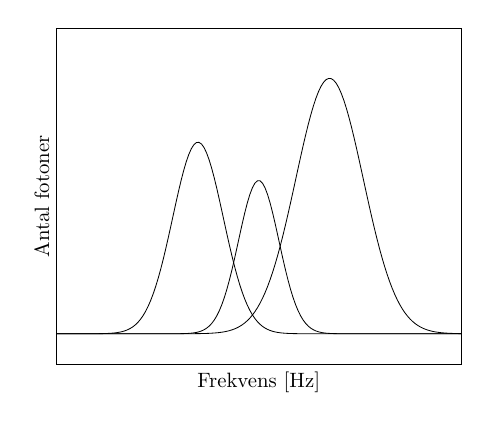
\begin{tikzpicture}[scale=0.75]
            \begin{axis}[
                ticks=none,
                ylabel=Antal fotoner, ylabel near ticks,
                xlabel={Frekvens [Hz]}, xlabel near ticks,
                xmin=-20, xmax=20,
                ymin=-1, ymax=10
            ]
                \addplot [domain=-25:25, samples=200, forget plot] {1/0.5*(2*pi)^0.5 * exp(-((x)^2)/2*0.25)};
                \addplot [domain=-25:25, samples=200, forget plot] {1/0.3*(2*pi)^0.5 * exp(-((x-7)^2)/2*0.09)};
                \addplot [domain=-25:25, samples=200, forget plot] {1/0.4*(2*pi)^0.5 * exp(-((x+6)^2)/2*0.16)};
            \end{axis}
        \end{tikzpicture}%
    }\qquad
    \subfloat[]{
        \centering
        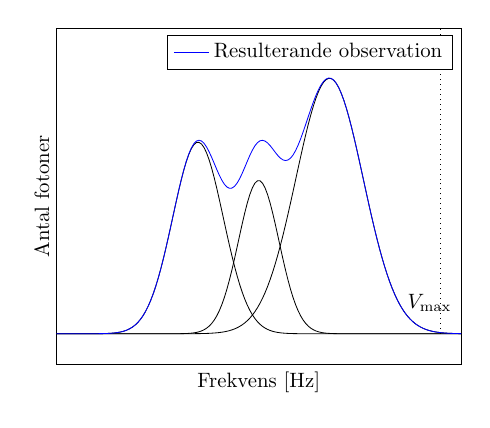
\begin{tikzpicture}[scale=0.75]
            \begin{axis}[
                ticks=none,
                ylabel=Antal fotoner, ylabel near ticks,
                xlabel={Frekvens [Hz]}, xlabel near ticks,
                xmin=-20, xmax=20,
                ymin=-1, ymax=10
            ]
                \addplot [domain=-25:25, samples=200, forget plot] {1/0.5*(2*pi)^0.5 * exp(-((x)^2)/2*0.25)};
                \addplot [domain=-25:25, samples=200, forget plot] {1/0.3*(2*pi)^0.5 * exp(-((x-7)^2)/2*0.09)};
                \addplot [domain=-25:25, samples=200, forget plot] {1/0.4*(2*pi)^0.5 * exp(-((x+6)^2)/2*0.16)};
                \addplot [blue,domain=-25:25, samples=200] {(1/0.5*(2*pi)^0.5 * exp(-((x)^2)/2*0.25)) + (1/0.3*(2*pi)^0.5 * exp(-((x-7)^2)/2*0.09)) + (1/0.4*(2*pi)^0.5 * exp(-((x+6)^2)/2*0.16))};
                \addlegendentry{Resulterande observation}
                \addplot [black, dotted] coordinates {
                    (18,0)
                    (18,12)
                };
                \coordinate [label=right:$V_{\mathrm{max}}$] (v-max) at (14,1);
            \end{axis}
        \end{tikzpicture}%
    }
    \caption{En exempelmätning med tre observerade vätemoln.}
    \label{fig:multiple_clouds}
\end{figure}

I figur \ref{fig:multiple_clouds}a har tre vätemoln observerats. I de fall mer än ett vätemoln observerats får observatören själv räkna ut hur många moln som observerats och hur de originella observationskurvorna såg ut, se figur \ref{fig:multiple_clouds}b.

\subsection{Koordinatsystem}
Många galaxer, även Vintergatan, har en skivform där merparten av den synliga massan återfinns längs med skivans plan. Det är möjligt att använda detta plan som bas för ett koordinatsystem där koordinaterna motsvarar en linje längs med alla tre dimensionerna\autocite{swin:galactic_coords}. Linjen vid longitud och latitud noll går genom Vintergatans mitt. Hela koordinatsystemet utgår från solsystemet. Se figur \ref{fig:galactic_coords}

\begin{figure}
    \centering
    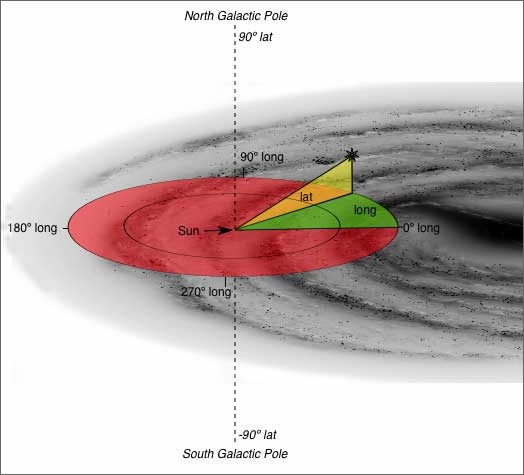
\includegraphics[width=0.8\textwidth]{pics/galactic_coords.jpg}
    \caption{Det galaktiska koordinatsystemet.}
    \label{fig:galactic_coords}
\end{figure}

\section{Syfte}
Syftet med den här rapporten är att besvara följande frågeställning: Hur ser Vintergatans galaktiska struktur ut? Därpå kommer vi även undersöka hur galaktiska strukturer uppstår, däremot kommer inget slutgiltigt svar att erbjudas på den andra frågan.
\chapter{Metod}

\section{Observationer}
Observationer genomfördes med radioteleskop vid Albanova under två separata tillfällen, kvällen 2018-09-19 och förmiddagen 2018-09-29. Teleskopet riktades successivt mot longituder med $5\degree$ mellanrum mellan $0\degree$ och $190\degree$ utefter det galaktiska koordinatsystemet. Latituden hölls konstant vid $0\degree$. Alla observationer gjordes under 90s och återfinns i bilaga 1.

Observationerna analyserades i två steg. I det första steget användes programmet xs\footnote{\url{http://satorchi.net/specsoft/specsoft.php}}, som utvecklades av forskare vid Chalmers för användning inom astrofysik, för att räkna ut de observerade molnens hastighet gentemot oss. I praktiken angavs gissningar till programmet, där programmet sedan anpassade kurvor till den data som fanns tillgänglig i förhållande till gissningarna. De anpassade kurvorna gav oss en genomsnittlig våglängd för fotoner från varje moln varpå programmet jämförde den förväntade våglängden med den uppmätta och räknade ut molnets relativa hastighet gentemot jorden samt storleken på en standardavvikelse. Vi noterade också den högsta uppmätta hastigheten $v_{\mathrm{max}}$ (se figur \ref{fig:multiple_clouds}b).

\begin{figure}
    \centering
    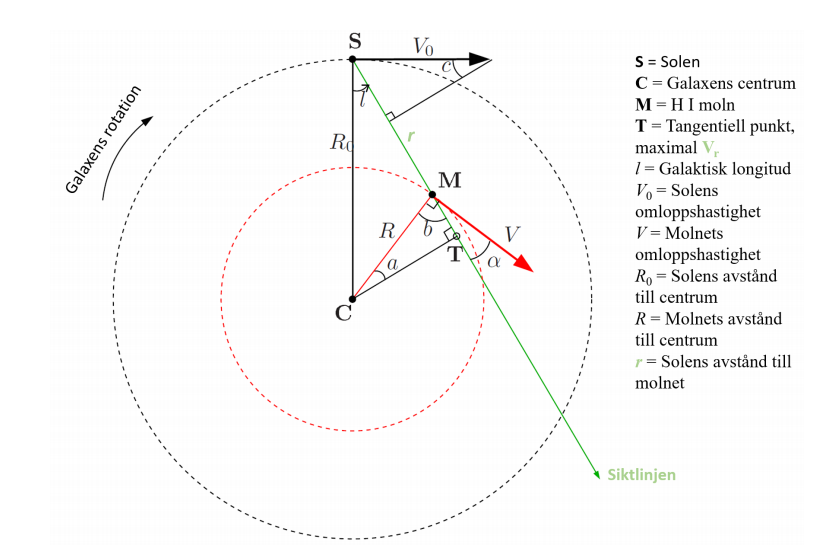
\includegraphics[width=\textwidth]{pics/trigonometri.png}
    \caption{Vintergatan ur ett trigonometriskt perspektiv.}
    \label{fig:trig}
\end{figure}

\section{Trigonometri}

Se figur \ref{fig:trig} för en schematisk ritning över Vintergatan ur ett trigonometriskt perspektiv.

För varje mätning vid en viss longitud $l$ antogs $v_{\mathrm{max}}$ (den maximalt uppmätta hastigheten) vara hastigheten i punkten $T$. Detta eftersom molnets hastighetsvektor $V$ går parallellt med siktlinjen.
För vätet i punkten $T$ antogs
\begin{equation*}
V = V_{\mathrm{max}} + V_{\mathrm{sol}} = V_{\mathrm{max}} + V_0 \cdot \mathrm{sin}(l),
\end{equation*}

där $V_0$ beskriver solens rotationshastighet kring galaxen och $V_{\mathrm{sol}}$ beskriver solens hastighet längs med siktlinjen, samt

\begin{equation*}
    \mathrm{sin}(l) = \frac{R}{R_0} \Rightarrow R = R_0 \cdot \mathrm{sin}(l).
\end{equation*}

Molnets hastighet relativt mot jorden ($V_R$) i punkten T sattes till $V \cdot \mathrm{cos}(\alpha) - V_0 \cdot \mathrm{sin}(c)$. $V \cdot \mathrm{cos}(\alpha)$ beskriver molnets hastighetskomposant i siktlinjen och $V_0 \cdot \mathrm{sin}(c)$ beskriver solens hastighetskomposant i siktlinjen.  Följande antogs:
\begin{gather*}
    90\degree - l = 180\degree - 90\degree - c \Rightarrow l = c \\
    \alpha = 90\degree - b \Rightarrow \mathrm{cos}(\alpha) = \mathrm{cos}(90\degree - b) = \mathrm{sin}(b) \\
    \lvert \mathrm{CT} \rvert = R \cdot \mathrm{sin}(b) = R_0 \cdot \mathrm{sin}(l) \Rightarrow \mathrm{sin}(b) = \frac{R_0}{R} \cdot \mathrm{sin}(l) \ (= \mathrm{cos}(\alpha))\\
\end{gather*}
Värdena på $\mathrm{cos}(\alpha)$ och $c$ sattes in för att lösa $V_R$.

\begin{equation*}
    V_R = V \cdot \mathrm{cos}(\alpha) - V_0 \cdot \mathrm{sin}(c) = V \cdot \frac{R_0}{R} \cdot \mathrm{sin}(l) - V_0 \cdot \mathrm{sin}(l)
\end{equation*}

Utifrån figur \ref{fig:rotation_our} som ritades upp antogs att rotationshastigheten V för allt väte, även det utanför punkten T, var konstant och lika stort som solens rotationshastighet $V_0$, ungefär 220 km/s.

\begin{figure}
    \centering
    \begin{tikzpicture}
        \begin{axis} [
            ylabel=$V_R$ (km/s), ylabel near ticks,
            xlabel=$R$ (kpc), xlabel near ticks,
            xticklabels={1,2,3,4,5,6,7,8,9},
            scale=0.75,
            label style={font=\small}
        ]
            \addplot [mark=*, smooth] table [col sep=comma] {Book1.csv};
        \end{axis}
    \end{tikzpicture}  
    \caption{$V_R$ med avseende på $R$ i punkten T för mätningar $0\degree \leq l \leq 90\degree.$}
    \label{fig:rotation_our}
\end{figure}

    %R = \frac{V_0 \cdot R_0 \cdot \mathrm{sin}(l)}{V_R + V_0 \cdot \mathrm{sin}(l)}


Cosinussatsen gav $R^2 = R_0^2 \cdot r \cdot \mathrm{cos}(l)$ och PQ-formeln gav \\$r = R_0 \cdot \mathrm{cos}(l) \pm \sqrt{R^2-R_0^2 \cdot \mathrm{sin}^2(l)}$.

För att konstruera en vetenskapligt acceptabel karta av dessa värden beaktades den felmariginal som undersökningen påverkades av. Vid användningen av dessa felmariginaler togs det hänsyn till till det faktum att de värden som led av felmarignalen gav upphov till nya värden; felen fortplantades därför genom hela undersökningen. Därför användes formlerna \ref{eq:eR} och \ref{eq:er}\autocite{wiki:fel} där $e_x$ defineras som felmarginalen för x. Felmarginalen för konstanterna $V_0$ och $R_0$ bortsågs då dessa värden är bestämda med mycket högre säkerhet än våra mätvärden.

\begin{equation} \label{eq:eR}
    \lvert e_R \rvert \leq \lvert \frac{R_0 \cdot V_0}{(V_R + V_0)^2} \rvert \cdot \lvert e_{V_r} \rvert
\end{equation}

\begin{equation} \label{eq:er}
    \lvert e_r \rvert \leq \lvert \frac{R}{\sqrt{R^2 - R_0^2 \cdot \mathrm{sin}^2(l)}} \rvert \cdot \lvert e_R \rvert
\end{equation}

%[2] förklara skillnaden mellan v_sol och v_0
\chapter{Resultat}

\begin{wrapfigure}{r}{0.7\textwidth}
    \centering
    \vspace{-40pt}
    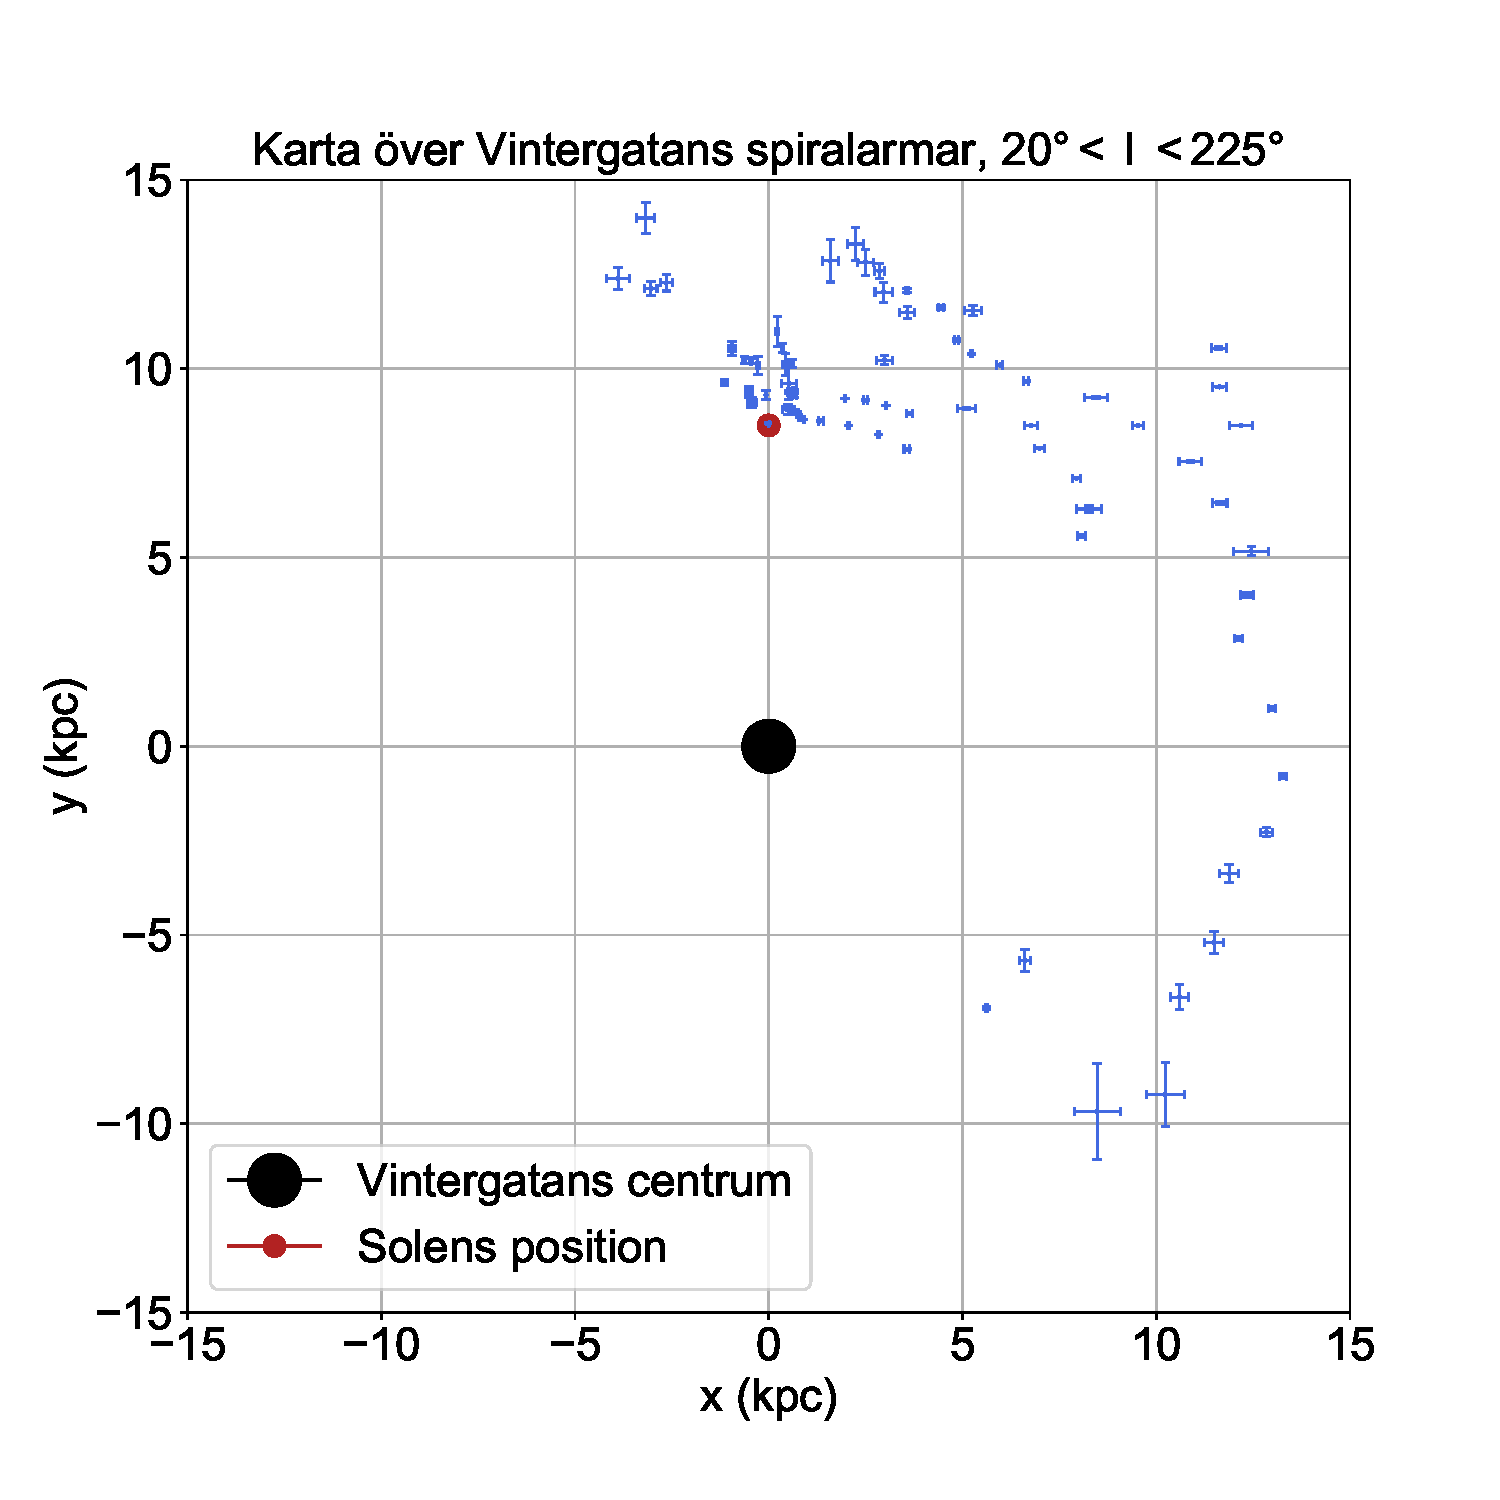
\includegraphics[max size={0.7\textwidth}{\textheight}]{pics/GustavVilhelm.pdf}
    %\vspace{20pt}
    \caption{Vår karta över Vintergatan}
    \label{fig:map_our}
\end{wrapfigure}

För varje mätning har vi nu två möjliga värden på r, avståndet mellan molnet och Vintergatans centrum. Om det ena värdet på r är negativt förkastar vi det och använder det positiva värdet som det ''riktiga'' värdet på r, men i det fall vi fick två positiva lösningar förkastade vi båda.

Utifrån de resulterande värdena ritade vi upp en karta över varje mätning, se figur \ref{fig:map_our}. Våra mätvärden och uträkningar återfinns i bilaga 1.
\chapter{Diskussion}
Resultatet vi fått verkar stämma överens med tidigare undersökningar, givet den spiralarm som vår karta avslöjar. Vintergatans struktur är numera allmän kunskap, och den kunskapen ligger i linje med de resultat detta arbete producerat\autocite{chalmers:samma_arbete}.

En brist med kartan vi ritade upp (figur \ref{fig:map_our}) är att vi förkastade mätvärden som gav upphov till två positiva lösningar på $r$. För att undvika detta kan man göra fler observationer vid samma longitud men variera latituden (man sveper med radioteleskopet ''upp och ner'' över det galaktiska planet). Om molnet befinner sig nära oss förväntas det synas vid latituder längre från $0\degree$ jämfört med om det är längre bort. Detta ansåg vi vara utanför vårt arbetes omfång men är något som framtida arbeten kan belysa vidare.

Denna del av rapporten kommer undersöka den andra delen av frågeställningen, nämligen varför galaktiska strukturer uppstår. De två ledande teorierna är ''Density Wave Theory'' och ''SSPSF''-modellen.

%density wave
Grundtanken med Density Wave Theory\autocite{swin.edu:density-wave} är att det i galaxer finns områden i omlopp kring ett masscentrum, i Vintergatans fall ett stort svart hål. Dessa områden har högre densitet, och i dessa områden trycks vätgas ihop vilket påbörjar processen som leder till att stjärnor uppstår. Dessa unga stjärnor lyser starkt vilket vi ser som ljusstarka spiralarmar. I dessa områden saktas även redan etablerade himlakroppar ner, vilket ger upphov till den förhöjda mängd stjärnor som återfinns där. 

På sjuttiotalet fann forskare att denna modell kunde appliceras på Saturnus ringar med förhållandevis lyckade resultat\autocite{wikipedia:density-wave}. Man fann likheter mellan förhållandet mellan Saturnus och dess ringar och förhållandet mellan vintergatans masscentrum och dess spiralarmar. Man behövde anpassa sambanden lite för att de ska passa den mycket mindre skalan, men likheterna styrker definitivt teorin.

%sspsf
En annan förelsagen förklaring är SSPSF-modellen \autocite{caltech:sspsf} som föreslår att galaxers struktur uppstår av chockvågor som uppstår av olika anledningar. Till skillnad mot Density Wave Theory går denna modell att applicera på alla former av galaxer.

Enligt SSPSF-modellen färdas ''tryckvågor'' genom galaxen som produceras av bland annat solvindar och supernovor. Dessa tryckvågor leder till att vätgas med större sannolikhet än vanligt trycks ihop och bildar nya stjärnor. (Stjärnor bildas när vätgas trycks ihop så pass mycket att dess egna gravitation drar till sig mer vätgas som ökar trycket så pass mycket att fusion uppstår).\autocite{nasa:star_formation} Tryckvågorna lämnar då bakom sig en högre koncentration av nya stjärnor, och eftersom nya stjärnor lyser starkare än äldre stjärnor är det möjligt att  urskilja diverse armstrukturer ur galaxer.

%jämför sspsf och density wave
Man kan konstatera att båda modellerna förlitar sig på ett område med förhållandevis högre täthet för att förklara stjärnornas strukturella formation. Density Wave Theory menar att områden med högre täthet färdas i omlopp runt en himmlakropp och att andra himlakroppar rör sig långsammare genom dessa områden. SSPSF-modellen menar att formationen uppstår på grund av tryckvågor - vilka genom sin natur medför högre täthet - som färdas genom universum. Skillnaden här är att SSPSF-modellens tryckvågor inte är bundna till ett omlopp, utan rör sig någorlunda fritt ur ett astronomiskt perpektiv, till skillnad mot de områden som Density Wave Theory beskriver.
\chapter{Sammanfattning}
I det här arbetet har vi kartlagt delar av Vintergatans galaktiska struktur och producerat en visualiserande karta över våra resultat. Vi har även diskuterat och jämfört två framstående teorier som försöker förklara hur galaktiska strukturer uppstår.

\section{Tack}
Vi skulle här vilja ta tillfället att tacka Tanja Nymark vid Vetenskapens Hus och Simon Eriksson vid Stockholms Universitets Astronomiska Institut för att möjligheten till denna studie erbjöds och handledning utdelades. Dessutom så uppskattades handledningen som vi fått av Karin Enström Salomonsson och Christina Kronlund vid Bromma Gymnasium och av Thomas Pettersson vid Blackebergs Gymnasium. Vi skulle även vilja tacka Miranda Jäderling för hjälpsam respons i opponeringen och ett intressant arbete att opponera på.

\chapter{Referenser}
\printbibliography[heading=none]

\section{Bilder}
\begin{description}
    \item [Figur \ref{fig:atmo_transparent}] \url{https://www.eso.org/public/usa/images/atm_opacity/}
    \item [Figur \ref{fig:galactic_coords}] \url{http://www.thinkastronomy.com/M13/Manual/common/galactic_coords.html}
    \item [Figur \ref{fig:trig}] \url{http://www.astro.lu.se/Education/utb/ASTA33/radiosweden_ht17.pdf}
\end{description}

\chapter{Bilaga}
\begin{description}
    \item [Våra mätvärden] är för stora för det här dokumentet så de återfinns på \url{http://v1.se/1b48}
\end{description}
\end{document}
